%!TEX TS-program = xelatex
%!TEX encoding = UTF-8 Unicode
% !TEX root = ../../metp.tex

\section{OSCILLATORE VIRTUALE}

L’oscillatore virtuale è un algoritmo che legge e invia in uscita,
ciclicamente, i campioni (dati quantizzati) di una forma d’onda.
Tutti i campioni che rappresentano un periodo della forma d’onda,
sono scritti precedentemente in un area di memoria chiamata tabella o table look-up.

Considerando il teorema del campionamento1 si possono seguire i seguenti passi per implementare un oscillatore virtuale:
1.- Si calcolano i valori dei campioni corrispondenti ad un ciclo della forma d’onda.
2.- Vengono memorizzati i valori in una tabella. Essa conterrà un ciclo di un' onda memorizzata in n locazioni di memoria. Ciascuna locazione è contrassegnata da un indice, indicato dai numeri interi.
3.- Si rileggono in sequenza i campioni, ciclicamente e ad un valore prefissato di frequenza di campionamento.


Obiettivi:

Implementing a sine oscillator from scratch in Faust
Understand the relation between the sine function and the generated sound
Use multiple sine oscillator to implement an additive synthesizer
Use SmartKeyboard to produce polyphonic mobile apps to control this synth

Referenze:
Manuale \emph{Faust}
computer music tutorial

\subsection{Funzione \emph{seno}}

\begin{figure}[ht]
  \centering
  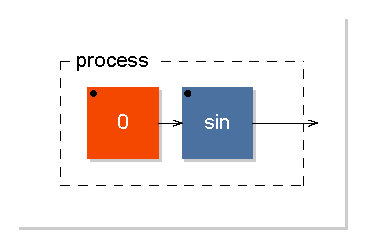
\includegraphics[]{CAPITOLI/0700/CODES/0701-seno-svg/process}
  \caption[]{Sine function. Faust Diagram.}
  \label{fdsine}
\end{figure}

\lstinputlisting{CAPITOLI/0700/CODES/0701-seno.dsp}

Questi sono i primi 5 campioni prodotti dalla formula $sin(0)$:

\lstinputlisting{CAPITOLI/0700/CODES/0701-seno.txt}

\lstinputlisting{CAPITOLI/0700/CODES/0702-senopi2.dsp}

Questi sono i primi 5 campioni prodotti dalla formula $sin(\pi/2)$:

\lstinputlisting{CAPITOLI/0700/CODES/0702-senopi2.txt}

questi i campioni

\lstinputlisting{CAPITOLI/0700/CODES/0703-senovariopi.txt}
